\begin{figure}[!htb]
  \centering
  \tikzsetnextfilenamesafe{Chapter5/3pb/mesh}
  \begin{tikzpicture}
    \node[inner sep=0] (mesh) at (0,0) {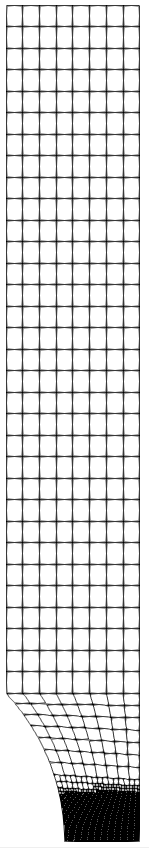
\includegraphics[width=0.09\textwidth,scale=0.5]{Chapter5/figures/3pb/mesh}};
    \node (box) at (mesh.south west) [draw,blue,thick,minimum width=0.09\textwidth,minimum height=51,anchor=south west] {};
    \node[inner sep=0] (meshzoom) at (7,0) {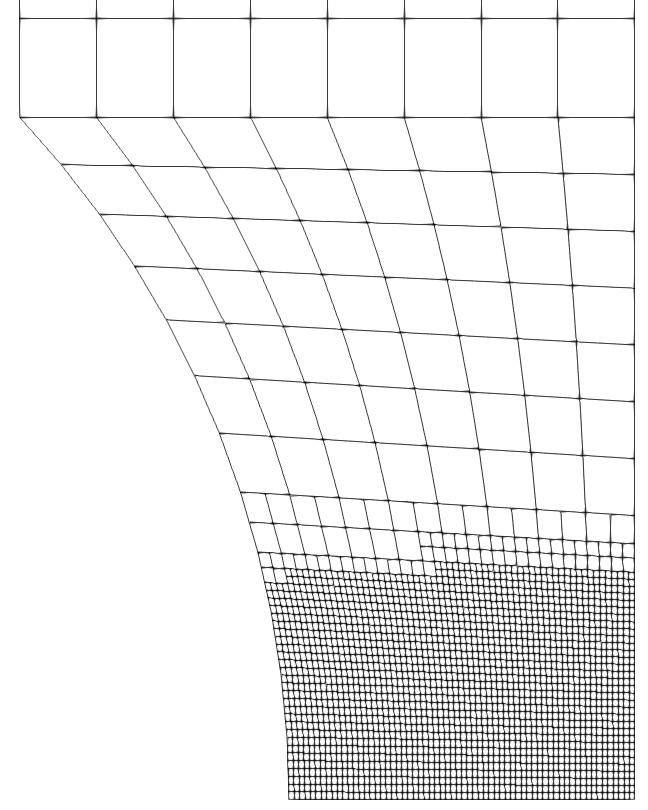
\includegraphics[width=0.36\textwidth,scale=0.5]{Chapter5/figures/3pb/mesh_zoom}};
    \node (boxzoom) at (meshzoom.south west) [draw,blue,thick,minimum width=0.36\textwidth,minimum height=195,anchor=south west] {};
    \draw (box.north east) -- (boxzoom.north west);
    \draw (box.south east) -- (boxzoom.south west);
  \end{tikzpicture}
  \caption{The mesh used for calibration and the zoomed-in view of the refined region.}
  \label{fig: Chapter5/3pb/mesh}
\end{figure}
